% Options for packages loaded elsewhere
\PassOptionsToPackage{unicode}{hyperref}
\PassOptionsToPackage{hyphens}{url}
%
\documentclass[
]{article}
\usepackage{amsmath,amssymb}
\usepackage{lmodern}
\usepackage{ifxetex,ifluatex}
\ifnum 0\ifxetex 1\fi\ifluatex 1\fi=0 % if pdftex
  \usepackage[T1]{fontenc}
  \usepackage[utf8]{inputenc}
  \usepackage{textcomp} % provide euro and other symbols
\else % if luatex or xetex
  \usepackage{unicode-math}
  \defaultfontfeatures{Scale=MatchLowercase}
  \defaultfontfeatures[\rmfamily]{Ligatures=TeX,Scale=1}
\fi
% Use upquote if available, for straight quotes in verbatim environments
\IfFileExists{upquote.sty}{\usepackage{upquote}}{}
\IfFileExists{microtype.sty}{% use microtype if available
  \usepackage[]{microtype}
  \UseMicrotypeSet[protrusion]{basicmath} % disable protrusion for tt fonts
}{}
\makeatletter
\@ifundefined{KOMAClassName}{% if non-KOMA class
  \IfFileExists{parskip.sty}{%
    \usepackage{parskip}
  }{% else
    \setlength{\parindent}{0pt}
    \setlength{\parskip}{6pt plus 2pt minus 1pt}}
}{% if KOMA class
  \KOMAoptions{parskip=half}}
\makeatother
\usepackage{xcolor}
\IfFileExists{xurl.sty}{\usepackage{xurl}}{} % add URL line breaks if available
\IfFileExists{bookmark.sty}{\usepackage{bookmark}}{\usepackage{hyperref}}
\hypersetup{
  pdftitle={Systematic Review of LDL Changes on a Ketogenic Diet},
  pdfauthor={Cody Cousineau and Dave Bridges},
  hidelinks,
  pdfcreator={LaTeX via pandoc}}
\urlstyle{same} % disable monospaced font for URLs
\usepackage[margin=1in]{geometry}
\usepackage{color}
\usepackage{fancyvrb}
\newcommand{\VerbBar}{|}
\newcommand{\VERB}{\Verb[commandchars=\\\{\}]}
\DefineVerbatimEnvironment{Highlighting}{Verbatim}{commandchars=\\\{\}}
% Add ',fontsize=\small' for more characters per line
\usepackage{framed}
\definecolor{shadecolor}{RGB}{248,248,248}
\newenvironment{Shaded}{\begin{snugshade}}{\end{snugshade}}
\newcommand{\AlertTok}[1]{\textcolor[rgb]{0.94,0.16,0.16}{#1}}
\newcommand{\AnnotationTok}[1]{\textcolor[rgb]{0.56,0.35,0.01}{\textbf{\textit{#1}}}}
\newcommand{\AttributeTok}[1]{\textcolor[rgb]{0.77,0.63,0.00}{#1}}
\newcommand{\BaseNTok}[1]{\textcolor[rgb]{0.00,0.00,0.81}{#1}}
\newcommand{\BuiltInTok}[1]{#1}
\newcommand{\CharTok}[1]{\textcolor[rgb]{0.31,0.60,0.02}{#1}}
\newcommand{\CommentTok}[1]{\textcolor[rgb]{0.56,0.35,0.01}{\textit{#1}}}
\newcommand{\CommentVarTok}[1]{\textcolor[rgb]{0.56,0.35,0.01}{\textbf{\textit{#1}}}}
\newcommand{\ConstantTok}[1]{\textcolor[rgb]{0.00,0.00,0.00}{#1}}
\newcommand{\ControlFlowTok}[1]{\textcolor[rgb]{0.13,0.29,0.53}{\textbf{#1}}}
\newcommand{\DataTypeTok}[1]{\textcolor[rgb]{0.13,0.29,0.53}{#1}}
\newcommand{\DecValTok}[1]{\textcolor[rgb]{0.00,0.00,0.81}{#1}}
\newcommand{\DocumentationTok}[1]{\textcolor[rgb]{0.56,0.35,0.01}{\textbf{\textit{#1}}}}
\newcommand{\ErrorTok}[1]{\textcolor[rgb]{0.64,0.00,0.00}{\textbf{#1}}}
\newcommand{\ExtensionTok}[1]{#1}
\newcommand{\FloatTok}[1]{\textcolor[rgb]{0.00,0.00,0.81}{#1}}
\newcommand{\FunctionTok}[1]{\textcolor[rgb]{0.00,0.00,0.00}{#1}}
\newcommand{\ImportTok}[1]{#1}
\newcommand{\InformationTok}[1]{\textcolor[rgb]{0.56,0.35,0.01}{\textbf{\textit{#1}}}}
\newcommand{\KeywordTok}[1]{\textcolor[rgb]{0.13,0.29,0.53}{\textbf{#1}}}
\newcommand{\NormalTok}[1]{#1}
\newcommand{\OperatorTok}[1]{\textcolor[rgb]{0.81,0.36,0.00}{\textbf{#1}}}
\newcommand{\OtherTok}[1]{\textcolor[rgb]{0.56,0.35,0.01}{#1}}
\newcommand{\PreprocessorTok}[1]{\textcolor[rgb]{0.56,0.35,0.01}{\textit{#1}}}
\newcommand{\RegionMarkerTok}[1]{#1}
\newcommand{\SpecialCharTok}[1]{\textcolor[rgb]{0.00,0.00,0.00}{#1}}
\newcommand{\SpecialStringTok}[1]{\textcolor[rgb]{0.31,0.60,0.02}{#1}}
\newcommand{\StringTok}[1]{\textcolor[rgb]{0.31,0.60,0.02}{#1}}
\newcommand{\VariableTok}[1]{\textcolor[rgb]{0.00,0.00,0.00}{#1}}
\newcommand{\VerbatimStringTok}[1]{\textcolor[rgb]{0.31,0.60,0.02}{#1}}
\newcommand{\WarningTok}[1]{\textcolor[rgb]{0.56,0.35,0.01}{\textbf{\textit{#1}}}}
\usepackage{longtable,booktabs,array}
\usepackage{calc} % for calculating minipage widths
% Correct order of tables after \paragraph or \subparagraph
\usepackage{etoolbox}
\makeatletter
\patchcmd\longtable{\par}{\if@noskipsec\mbox{}\fi\par}{}{}
\makeatother
% Allow footnotes in longtable head/foot
\IfFileExists{footnotehyper.sty}{\usepackage{footnotehyper}}{\usepackage{footnote}}
\makesavenoteenv{longtable}
\usepackage{graphicx}
\makeatletter
\def\maxwidth{\ifdim\Gin@nat@width>\linewidth\linewidth\else\Gin@nat@width\fi}
\def\maxheight{\ifdim\Gin@nat@height>\textheight\textheight\else\Gin@nat@height\fi}
\makeatother
% Scale images if necessary, so that they will not overflow the page
% margins by default, and it is still possible to overwrite the defaults
% using explicit options in \includegraphics[width, height, ...]{}
\setkeys{Gin}{width=\maxwidth,height=\maxheight,keepaspectratio}
% Set default figure placement to htbp
\makeatletter
\def\fps@figure{htbp}
\makeatother
\setlength{\emergencystretch}{3em} % prevent overfull lines
\providecommand{\tightlist}{%
  \setlength{\itemsep}{0pt}\setlength{\parskip}{0pt}}
\setcounter{secnumdepth}{-\maxdimen} % remove section numbering
\ifluatex
  \usepackage{selnolig}  % disable illegal ligatures
\fi

\title{Systematic Review of LDL Changes on a Ketogenic Diet}
\author{Cody Cousineau and Dave Bridges}
\date{June 18, 2021}

\begin{document}
\maketitle

{
\setcounter{tocdepth}{2}
\tableofcontents
}
= \# Purpose

To evaluate how LDL changes in ketogenic diet studies

\hypertarget{experimental-details}{%
\section{Experimental Details}\label{experimental-details}}

Evaluated studies where ketogenic diets (\textless25g/day of CHO) are
used and weight and LDL-C are reported as an outcome

\hypertarget{raw-data}{%
\section{Raw Data}\label{raw-data}}

Reviewed data from the Choi \emph{et al} meta-analysis
(\url{http://dx.doi.org/10.3390/nu12072005}), pulling in data on
baseline weight, weight changes, LDL, LDL changes and standard
deviations. A systematic literature search of PubMed was then performed
to identify other randomized controlled trials (RCTs) and single-arm
interventions of patients that evaluated the effects of a ketogenic diet
on weight and lipid profile as primary endpoints. All studies using a KD
diet that met our inclusion criteria where intake of carbohydrate was
less than 25 grams per day were included. This search was most recently
updated on xxx.

\begin{Shaded}
\begin{Highlighting}[]
\FunctionTok{library}\NormalTok{(readxl) }\CommentTok{\#loads the readr package}
\NormalTok{filename }\OtherTok{\textless{}{-}} \StringTok{\textquotesingle{}LDL Study Summary.xlsx\textquotesingle{}} \CommentTok{\#make this a separate line, you can use any variable you want}

\CommentTok{\#this loads whatever the file is into a dataframe called exp.data if it exists}
\NormalTok{exp.data }\OtherTok{\textless{}{-}} \FunctionTok{read\_excel}\NormalTok{(filename)}
\NormalTok{eval.data }\OtherTok{\textless{}{-}}\NormalTok{ exp.data }\SpecialCharTok{\%\textgreater{}\%} 
  \FunctionTok{filter}\NormalTok{(Use}\SpecialCharTok{==}\StringTok{\textquotesingle{}x\textquotesingle{}}\NormalTok{) }\SpecialCharTok{\%\textgreater{}\%}
  \FunctionTok{mutate}\NormalTok{(}\AttributeTok{Pct.Wt.Change =} \StringTok{\textasciigrave{}}\AttributeTok{Weight Change}\StringTok{\textasciigrave{}}\SpecialCharTok{/}\StringTok{\textasciigrave{}}\AttributeTok{Baseline Weight}\StringTok{\textasciigrave{}}\SpecialCharTok{*}\DecValTok{100}\NormalTok{)}\SpecialCharTok{\%\textgreater{}\%}
  \FunctionTok{mutate}\NormalTok{(}\AttributeTok{PCT.BMI.Change =} \StringTok{\textasciigrave{}}\AttributeTok{BMI Change}\StringTok{\textasciigrave{}} \SpecialCharTok{/} \StringTok{\textasciigrave{}}\AttributeTok{Baseline BMI}\StringTok{\textasciigrave{}}\SpecialCharTok{*}\DecValTok{100}\NormalTok{)}\SpecialCharTok{\%\textgreater{}\%}
  \FunctionTok{mutate}\NormalTok{(}\AttributeTok{Sex.Group =} \FunctionTok{cut}\NormalTok{(}\StringTok{\textasciigrave{}}\AttributeTok{Percent Male}\StringTok{\textasciigrave{}}\NormalTok{, }\AttributeTok{breaks =} \FunctionTok{c}\NormalTok{(}\DecValTok{0}\NormalTok{,.}\DecValTok{1}\NormalTok{,.}\DecValTok{9}\NormalTok{,}\DecValTok{1}\NormalTok{), }\AttributeTok{include.lowest =} \ConstantTok{TRUE}\NormalTok{, }\AttributeTok{labels =} \FunctionTok{c}\NormalTok{(}\StringTok{"Mostly Female"}\NormalTok{, }\StringTok{"Mixed"}\NormalTok{, }\StringTok{"Mostly Male"}\NormalTok{)))}
\end{Highlighting}
\end{Shaded}

These data can be found in
\textbf{C:/Users/Cody/Documents/GitHub/PrecisionNutrition/Meta Analysis}
in a file named \textbf{LDL Study Summary.xlsx}. This script was most
recently updated on \textbf{Wed Apr 06 10:17:41 2022}.

\hypertarget{analysis}{%
\section{Analysis}\label{analysis}}

\hypertarget{variance-in-ldl-c}{%
\section{Variance in LDL-C}\label{variance-in-ldl-c}}

\begin{Shaded}
\begin{Highlighting}[]
\FunctionTok{library}\NormalTok{(ggplot2)}

\NormalTok{eval.data }\OtherTok{\textless{}{-}}
\NormalTok{  eval.data }\SpecialCharTok{\%\textgreater{}\%}
  \FunctionTok{mutate}\NormalTok{(}\AttributeTok{LDL.endpoint =} \StringTok{\textasciigrave{}}\AttributeTok{Baseline LDL}\StringTok{\textasciigrave{}}\SpecialCharTok{+}\StringTok{\textasciigrave{}}\AttributeTok{Change in LDL{-}C}\StringTok{\textasciigrave{}}\NormalTok{)}

\NormalTok{eval.data }\SpecialCharTok{\%\textgreater{}\%}
  \FunctionTok{filter}\NormalTok{(}\SpecialCharTok{!}\NormalTok{(}\FunctionTok{is.na}\NormalTok{(}\StringTok{\textasciigrave{}}\AttributeTok{Endpoint SD}\StringTok{\textasciigrave{}}\NormalTok{))) }\SpecialCharTok{\%\textgreater{}\%}
  \FunctionTok{ggplot}\NormalTok{(}\FunctionTok{aes}\NormalTok{(}\AttributeTok{y=}\NormalTok{LDL.endpoint,}
             \AttributeTok{ymin=}\NormalTok{LDL.endpoint}\SpecialCharTok{{-}}\StringTok{\textasciigrave{}}\AttributeTok{Endpoint SD}\StringTok{\textasciigrave{}}\NormalTok{,}
             \AttributeTok{ymax=}\NormalTok{LDL.endpoint}\SpecialCharTok{+}\StringTok{\textasciigrave{}}\AttributeTok{Endpoint SD}\StringTok{\textasciigrave{}}\NormalTok{,}
             \AttributeTok{x=}\FunctionTok{reorder}\NormalTok{(Study,}\SpecialCharTok{{-}}\StringTok{\textasciigrave{}}\AttributeTok{LDL.endpoint}\StringTok{\textasciigrave{}}\NormalTok{ ))) }\SpecialCharTok{+}
  \FunctionTok{geom\_point}\NormalTok{() }\SpecialCharTok{+}
  \FunctionTok{geom\_errorbar}\NormalTok{()}\SpecialCharTok{+}
  \FunctionTok{theme}\NormalTok{(}\AttributeTok{axis.text.x =} \FunctionTok{element\_text}\NormalTok{(}\AttributeTok{angle =} \DecValTok{45}\NormalTok{, }\AttributeTok{vjust =} \FloatTok{0.5}\NormalTok{, }\AttributeTok{hjust=}\DecValTok{1}\NormalTok{))}
\end{Highlighting}
\end{Shaded}

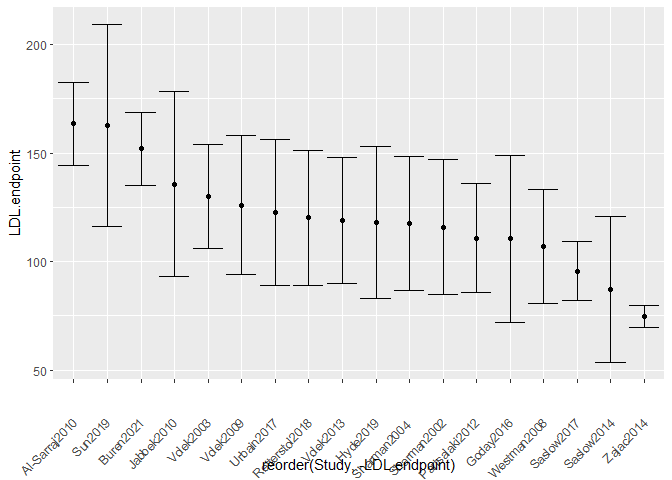
\includegraphics{figures/ldlc-endpoint-1.png}

\begin{Shaded}
\begin{Highlighting}[]
\NormalTok{eval.data }\SpecialCharTok{\%\textgreater{}\%} 
  \FunctionTok{summarize\_at}\NormalTok{(}\AttributeTok{.vars=}\FunctionTok{vars}\NormalTok{(Pct.Wt.Change,}\StringTok{\textasciigrave{}}\AttributeTok{Weight Change}\StringTok{\textasciigrave{}}\NormalTok{,}\StringTok{\textasciigrave{}}\AttributeTok{Change in LDL{-}C}\StringTok{\textasciigrave{}}\NormalTok{),}
               \AttributeTok{.funs=}\FunctionTok{funs}\NormalTok{(mean)) }
\end{Highlighting}
\end{Shaded}

\begin{verbatim}
## # A tibble: 1 x 3
##   Pct.Wt.Change `Weight Change` `Change in LDL-C`
##           <dbl>           <dbl>             <dbl>
## 1            NA              NA              11.4
\end{verbatim}

\hypertarget{meta-analysis}{%
\section{Meta-Analysis}\label{meta-analysis}}

\begin{Shaded}
\begin{Highlighting}[]
\NormalTok{meta.data }\OtherTok{\textless{}{-}}
\NormalTok{  eval.data }\SpecialCharTok{\%\textgreater{}\%}
  \FunctionTok{filter}\NormalTok{(}\SpecialCharTok{!}\FunctionTok{is.na}\NormalTok{(}\StringTok{\textasciigrave{}}\AttributeTok{Endpoint SD}\StringTok{\textasciigrave{}}\NormalTok{)) }\SpecialCharTok{\%\textgreater{}\%}
  \FunctionTok{mutate}\NormalTok{(}\AttributeTok{Pooled.SD=}\FunctionTok{sqrt}\NormalTok{(}\StringTok{\textasciigrave{}}\AttributeTok{Baseline SD}\StringTok{\textasciigrave{}}\SpecialCharTok{\^{}}\DecValTok{2}\SpecialCharTok{+}\StringTok{\textasciigrave{}}\AttributeTok{Endpoint SD}\StringTok{\textasciigrave{}}\SpecialCharTok{\^{}}\DecValTok{2}\NormalTok{)) }\SpecialCharTok{\%\textgreater{}\%}
  \FunctionTok{mutate}\NormalTok{(}\AttributeTok{SMD=}\StringTok{\textasciigrave{}}\AttributeTok{Change in LDL{-}C}\StringTok{\textasciigrave{}}\NormalTok{) }\SpecialCharTok{\%\textgreater{}\%}
  \FunctionTok{mutate}\NormalTok{(}\AttributeTok{SMD.Wt =} \StringTok{\textasciigrave{}}\AttributeTok{Weight Change}\StringTok{\textasciigrave{}}\NormalTok{) }

\FunctionTok{library}\NormalTok{(meta)}
\NormalTok{ldl.c.meta }\OtherTok{\textless{}{-}} \FunctionTok{metagen}\NormalTok{(}\AttributeTok{TE =}\NormalTok{ SMD,}
                 \AttributeTok{seTE =}\NormalTok{ Pooled.SD,}
                 \AttributeTok{n.e=}\NormalTok{n,}
                 \AttributeTok{n.c=}\NormalTok{n,}
                 \AttributeTok{studlab =}\NormalTok{ Study,}
                 \AttributeTok{data =}\NormalTok{ meta.data,}
                 \AttributeTok{sm =} \StringTok{"SMD"}\NormalTok{,}
                 \AttributeTok{comb.fixed =} \ConstantTok{TRUE}\NormalTok{,}
                 \AttributeTok{comb.random =} \ConstantTok{FALSE}\NormalTok{,}
                 \CommentTok{\#method.tau = "REML",}
                 \AttributeTok{hakn =} \ConstantTok{TRUE}\NormalTok{,}
                 \AttributeTok{title =} \StringTok{"LDL{-}C Changes in Ketogenic Diet Studies"}\NormalTok{)}

\FunctionTok{forest.meta}\NormalTok{(ldl.c.meta, }
            \AttributeTok{sortvar =}\NormalTok{ SMD,}
            \AttributeTok{predict =}\NormalTok{ F, }
            \AttributeTok{print.tau2 =} \ConstantTok{TRUE}\NormalTok{,}
            \AttributeTok{print.I2 =} \ConstantTok{TRUE}\NormalTok{,}
            \CommentTok{\#leftcols=c(\textquotesingle{}Study\textquotesingle{}),}
            \CommentTok{\#rightlabs=c(\textquotesingle{}Change\textquotesingle{},\textquotesingle{}95\% CI\textquotesingle{},\textquotesingle{}Weight\textquotesingle{}),}
            \AttributeTok{layout =} \StringTok{"RevMan5"}\NormalTok{,}
            \AttributeTok{fontsize=}\DecValTok{8}\NormalTok{,}
            \AttributeTok{leftcols =} \FunctionTok{c}\NormalTok{(}\StringTok{"Study"}\NormalTok{,}\StringTok{\textquotesingle{}effect\textquotesingle{}}\NormalTok{,}\StringTok{"seTE"}\NormalTok{,}\StringTok{\textquotesingle{}ci\textquotesingle{}}\NormalTok{,}\StringTok{\textquotesingle{}w.fixed\textquotesingle{}}\NormalTok{),}
            \AttributeTok{leftlabs =} \FunctionTok{c}\NormalTok{(}\StringTok{"Study"}\NormalTok{,}\StringTok{"Change"}\NormalTok{,}\StringTok{"SE"}\NormalTok{,}\StringTok{"95\% CI"}\NormalTok{,}\StringTok{"Weight"}\NormalTok{),}
            \AttributeTok{range =}\NormalTok{ F,}
            \AttributeTok{digits=}\DecValTok{1}\NormalTok{,}
            \AttributeTok{digits.se=}\DecValTok{1}\NormalTok{)}
\end{Highlighting}
\end{Shaded}

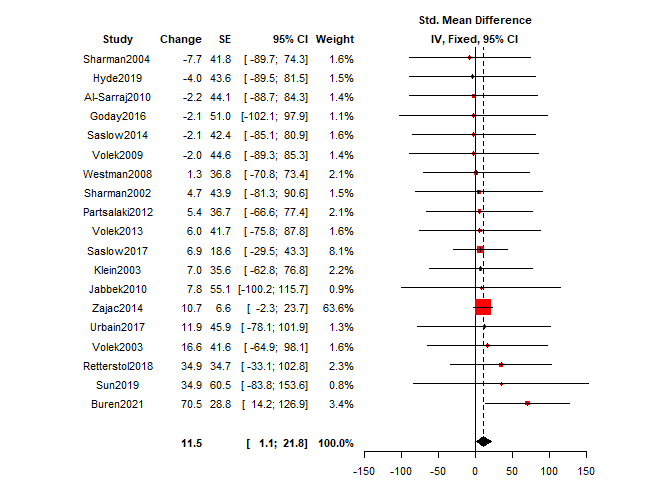
\includegraphics{figures/meta-analysis-1.png}

\hypertarget{average-change-in-ldl-c}{%
\section{Average Change in LDL-C}\label{average-change-in-ldl-c}}

\begin{Shaded}
\begin{Highlighting}[]
\NormalTok{eval.data }\SpecialCharTok{\%\textgreater{}\%}
  \FunctionTok{ggplot}\NormalTok{(}\FunctionTok{aes}\NormalTok{(}\AttributeTok{y=}\StringTok{\textasciigrave{}}\AttributeTok{Change in LDL{-}C}\StringTok{\textasciigrave{}}\NormalTok{,}
             \AttributeTok{x=}\FunctionTok{reorder}\NormalTok{(Study, }\SpecialCharTok{{-}}\StringTok{\textasciigrave{}}\AttributeTok{Change in LDL{-}C}\StringTok{\textasciigrave{}}\NormalTok{))) }\SpecialCharTok{+}
  \FunctionTok{geom\_bar}\NormalTok{(}\AttributeTok{stat=}\StringTok{\textquotesingle{}identity\textquotesingle{}}\NormalTok{) }\SpecialCharTok{+}
  \FunctionTok{labs}\NormalTok{(}\AttributeTok{x=}\StringTok{"Study"}\NormalTok{)}
\end{Highlighting}
\end{Shaded}

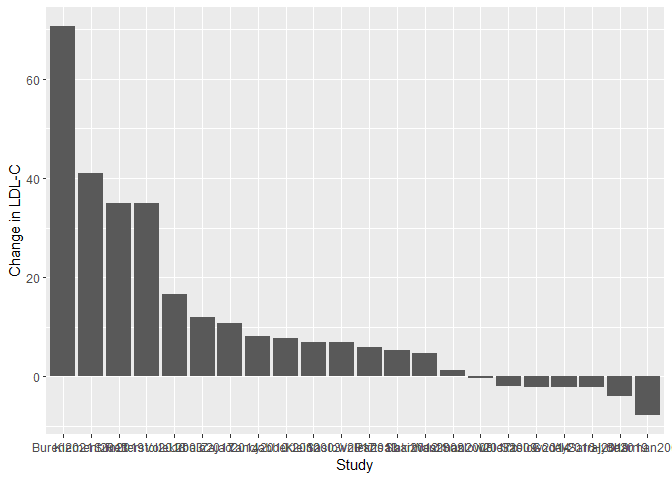
\includegraphics{figures/ldl-change-1.png}

\begin{Shaded}
\begin{Highlighting}[]
\NormalTok{eval.data }\SpecialCharTok{\%\textgreater{}\%}
  \FunctionTok{ggplot}\NormalTok{(}\FunctionTok{aes}\NormalTok{(}\AttributeTok{y=}\StringTok{\textasciigrave{}}\AttributeTok{Change in LDL{-}C}\StringTok{\textasciigrave{}}\NormalTok{,}
             \AttributeTok{x=}\FunctionTok{reorder}\NormalTok{(Study, }\SpecialCharTok{{-}}\StringTok{\textasciigrave{}}\AttributeTok{Change in LDL{-}C}\StringTok{\textasciigrave{}}\NormalTok{))) }\SpecialCharTok{+}
  \FunctionTok{geom\_bar}\NormalTok{(}\AttributeTok{stat=}\StringTok{\textquotesingle{}identity\textquotesingle{}}\NormalTok{, }\FunctionTok{aes}\NormalTok{(}\AttributeTok{fill=}\StringTok{\textasciigrave{}}\AttributeTok{Percent Male}\StringTok{\textasciigrave{}}\NormalTok{)) }\SpecialCharTok{+}
  \FunctionTok{labs}\NormalTok{(}\AttributeTok{x=}\StringTok{"Study"}\NormalTok{)}\SpecialCharTok{+}
    \FunctionTok{theme}\NormalTok{(}\AttributeTok{axis.text.x =} \FunctionTok{element\_text}\NormalTok{(}\AttributeTok{angle =} \DecValTok{45}\NormalTok{, }\AttributeTok{vjust =} \FloatTok{0.5}\NormalTok{, }\AttributeTok{hjust=}\DecValTok{1}\NormalTok{))}
\end{Highlighting}
\end{Shaded}

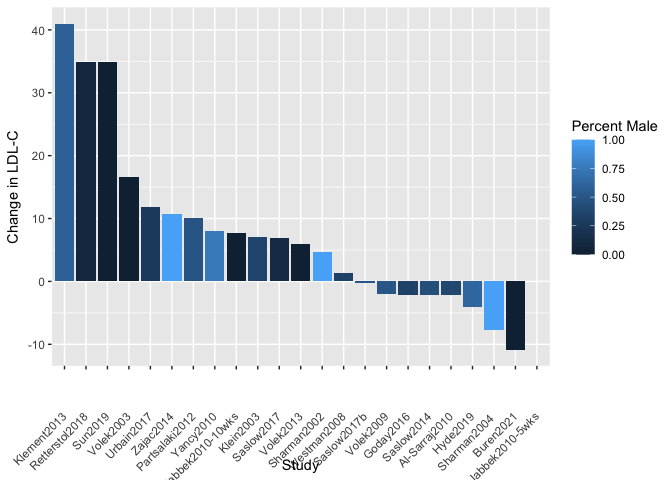
\includegraphics{figures/ldl-change-2.png}

\begin{Shaded}
\begin{Highlighting}[]
\NormalTok{eval.data }\SpecialCharTok{\%\textgreater{}\%}
  \FunctionTok{ggplot}\NormalTok{(}\FunctionTok{aes}\NormalTok{(}\AttributeTok{y=}\StringTok{\textasciigrave{}}\AttributeTok{Change in LDL{-}C}\StringTok{\textasciigrave{}}\NormalTok{,}
             \AttributeTok{x=}\FunctionTok{reorder}\NormalTok{(Study, }\SpecialCharTok{{-}}\StringTok{\textasciigrave{}}\AttributeTok{Change in LDL{-}C}\StringTok{\textasciigrave{}}\NormalTok{))) }\SpecialCharTok{+}
  \FunctionTok{geom\_bar}\NormalTok{(}\AttributeTok{stat=}\StringTok{\textquotesingle{}identity\textquotesingle{}}\NormalTok{, }\FunctionTok{aes}\NormalTok{(}\AttributeTok{fill=}\StringTok{\textasciigrave{}}\AttributeTok{Sex.Group}\StringTok{\textasciigrave{}}\NormalTok{)) }\SpecialCharTok{+}
  \FunctionTok{labs}\NormalTok{(}\AttributeTok{x=}\StringTok{"Study"}\NormalTok{) }\SpecialCharTok{+}
    \FunctionTok{theme}\NormalTok{(}\AttributeTok{axis.text.x =} \FunctionTok{element\_text}\NormalTok{(}\AttributeTok{angle =} \DecValTok{45}\NormalTok{, }\AttributeTok{vjust =} \FloatTok{0.5}\NormalTok{, }\AttributeTok{hjust=}\DecValTok{1}\NormalTok{))}
\end{Highlighting}
\end{Shaded}

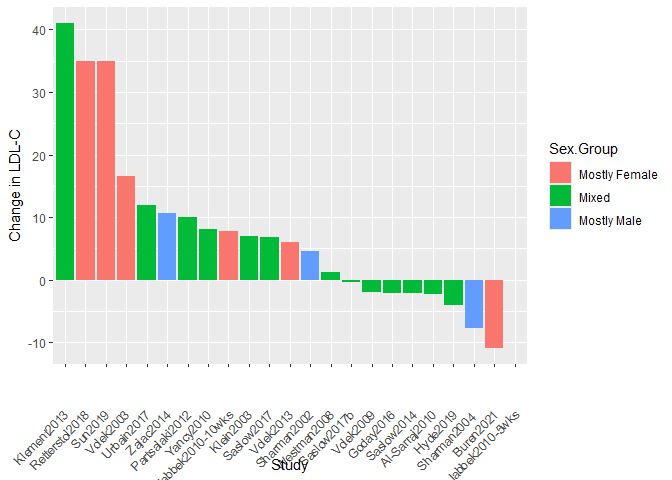
\includegraphics{figures/ldl-change-3.png}

\hypertarget{relative-to-weight}{%
\subsection{Relative to Weight}\label{relative-to-weight}}

\begin{Shaded}
\begin{Highlighting}[]
\FunctionTok{library}\NormalTok{(ggrepel)}
\FunctionTok{library}\NormalTok{(ggplot2)}
\NormalTok{eval.data }\SpecialCharTok{\%\textgreater{}\%}
  \FunctionTok{ggplot}\NormalTok{(}\FunctionTok{aes}\NormalTok{(}\AttributeTok{y=}\StringTok{\textasciigrave{}}\AttributeTok{Change in LDL{-}C}\StringTok{\textasciigrave{}}\NormalTok{,}
             \AttributeTok{x=}\StringTok{\textasciigrave{}}\AttributeTok{Baseline Weight}\StringTok{\textasciigrave{}}\NormalTok{)) }\SpecialCharTok{+}
  \FunctionTok{geom\_point}\NormalTok{() }\SpecialCharTok{+}
  \FunctionTok{geom\_smooth}\NormalTok{(}\AttributeTok{span=}\DecValTok{1}\NormalTok{) }\SpecialCharTok{+}
  \FunctionTok{geom\_text\_repel}\NormalTok{(}\FunctionTok{aes}\NormalTok{(}\AttributeTok{label=}\NormalTok{Study)) }\SpecialCharTok{+}
  \FunctionTok{labs}\NormalTok{(}\AttributeTok{x=}\StringTok{"Baseline Weight"}\NormalTok{)}
\end{Highlighting}
\end{Shaded}

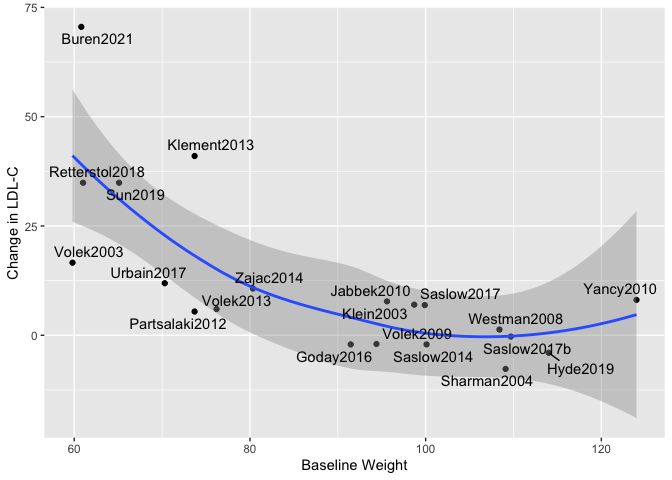
\includegraphics{figures/ldl-change-vs-weight-1.png}

\begin{Shaded}
\begin{Highlighting}[]
\NormalTok{eval.data }\SpecialCharTok{\%\textgreater{}\%}
  \FunctionTok{ggplot}\NormalTok{(}\FunctionTok{aes}\NormalTok{(}\AttributeTok{y=}\StringTok{\textasciigrave{}}\AttributeTok{Change in LDL{-}C}\StringTok{\textasciigrave{}}\NormalTok{,}
             \AttributeTok{x=}\StringTok{\textasciigrave{}}\AttributeTok{Baseline BMI}\StringTok{\textasciigrave{}}\NormalTok{)) }\SpecialCharTok{+}
  \FunctionTok{geom\_point}\NormalTok{() }\SpecialCharTok{+}
  \FunctionTok{geom\_smooth}\NormalTok{(}\AttributeTok{span=}\DecValTok{1}\NormalTok{) }\SpecialCharTok{+}
  \FunctionTok{geom\_text\_repel}\NormalTok{(}\FunctionTok{aes}\NormalTok{(}\AttributeTok{label=}\NormalTok{Study)) }\SpecialCharTok{+}
  \FunctionTok{labs}\NormalTok{(}\AttributeTok{x=}\StringTok{"Baseline BMI"}\NormalTok{)}
\end{Highlighting}
\end{Shaded}

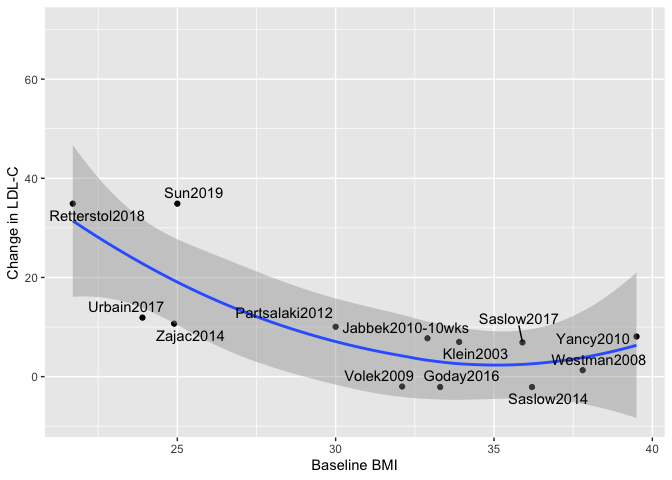
\includegraphics{figures/ldl-change-vs-weight-2.png}

\begin{Shaded}
\begin{Highlighting}[]
\NormalTok{eval.data }\SpecialCharTok{\%\textgreater{}\%}
  \FunctionTok{ggplot}\NormalTok{(}\FunctionTok{aes}\NormalTok{(}\AttributeTok{y=}\StringTok{\textasciigrave{}}\AttributeTok{Change in LDL{-}C}\StringTok{\textasciigrave{}}\NormalTok{,}
             \AttributeTok{x=}\StringTok{\textasciigrave{}}\AttributeTok{Baseline Weight}\StringTok{\textasciigrave{}}\NormalTok{)) }\SpecialCharTok{+}
  \FunctionTok{geom\_point}\NormalTok{() }\SpecialCharTok{+}
  \FunctionTok{geom\_smooth}\NormalTok{(}\AttributeTok{method=}\StringTok{\textquotesingle{}lm\textquotesingle{}}\NormalTok{) }\SpecialCharTok{+}
  \FunctionTok{geom\_text\_repel}\NormalTok{(}\FunctionTok{aes}\NormalTok{(}\AttributeTok{label=}\NormalTok{Study)) }\SpecialCharTok{+}
  \FunctionTok{labs}\NormalTok{(}\AttributeTok{x=}\StringTok{"Baseline Weight"}\NormalTok{)}
\end{Highlighting}
\end{Shaded}

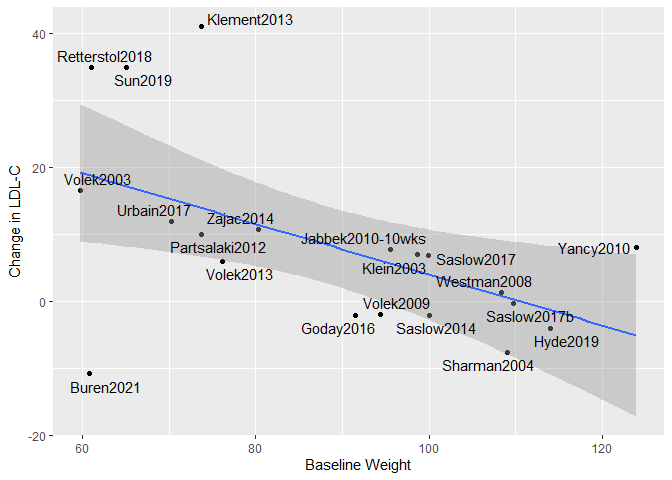
\includegraphics{figures/ldl-change-vs-weight-3.png}

\begin{Shaded}
\begin{Highlighting}[]
\NormalTok{eval.data }\SpecialCharTok{\%\textgreater{}\%}
  \FunctionTok{ggplot}\NormalTok{(}\FunctionTok{aes}\NormalTok{(}\AttributeTok{y=}\StringTok{\textasciigrave{}}\AttributeTok{Change in LDL{-}C}\StringTok{\textasciigrave{}}\NormalTok{,}
             \AttributeTok{x=}\StringTok{\textasciigrave{}}\AttributeTok{Baseline BMI}\StringTok{\textasciigrave{}}\NormalTok{)) }\SpecialCharTok{+}
  \FunctionTok{geom\_point}\NormalTok{() }\SpecialCharTok{+}
  \FunctionTok{geom\_smooth}\NormalTok{(}\AttributeTok{method=}\StringTok{\textquotesingle{}lm\textquotesingle{}}\NormalTok{) }\SpecialCharTok{+}
  \FunctionTok{geom\_text\_repel}\NormalTok{(}\FunctionTok{aes}\NormalTok{(}\AttributeTok{label=}\NormalTok{Study)) }\SpecialCharTok{+}
  \FunctionTok{labs}\NormalTok{(}\AttributeTok{x=}\StringTok{"Baseline BMI"}\NormalTok{)}
\end{Highlighting}
\end{Shaded}

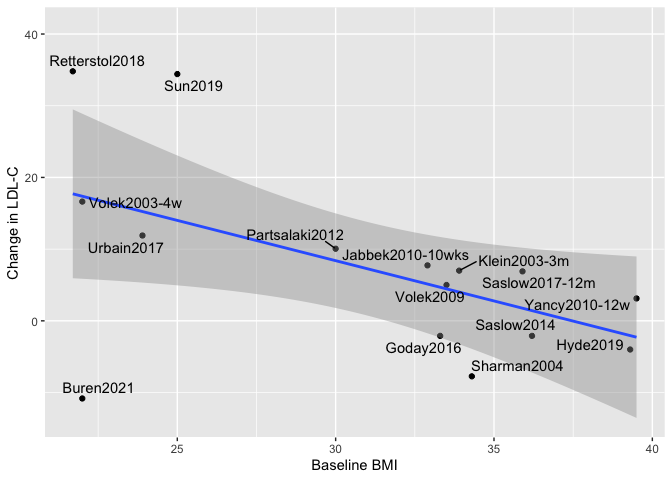
\includegraphics{figures/ldl-change-vs-weight-4.png}

\begin{Shaded}
\begin{Highlighting}[]
\NormalTok{eval.data }\SpecialCharTok{\%\textgreater{}\%}
  \FunctionTok{ggplot}\NormalTok{(}\FunctionTok{aes}\NormalTok{(}\AttributeTok{y=}\StringTok{\textasciigrave{}}\AttributeTok{Change in LDL{-}C}\StringTok{\textasciigrave{}}\NormalTok{,}
             \AttributeTok{x=}\StringTok{\textasciigrave{}}\AttributeTok{Baseline Weight}\StringTok{\textasciigrave{}}\NormalTok{,}
             \AttributeTok{col=}\StringTok{\textasciigrave{}}\AttributeTok{Percent Male}\StringTok{\textasciigrave{}}\NormalTok{)) }\SpecialCharTok{+}
  \FunctionTok{geom\_point}\NormalTok{() }\SpecialCharTok{+}
  \FunctionTok{geom\_smooth}\NormalTok{(}\AttributeTok{method=}\StringTok{\textquotesingle{}lm\textquotesingle{}}\NormalTok{) }\SpecialCharTok{+}
  \FunctionTok{geom\_text\_repel}\NormalTok{(}\FunctionTok{aes}\NormalTok{(}\AttributeTok{label=}\NormalTok{Study)) }\SpecialCharTok{+}
  \FunctionTok{labs}\NormalTok{(}\AttributeTok{x=}\StringTok{"Baseline Weight"}\NormalTok{)}
\end{Highlighting}
\end{Shaded}

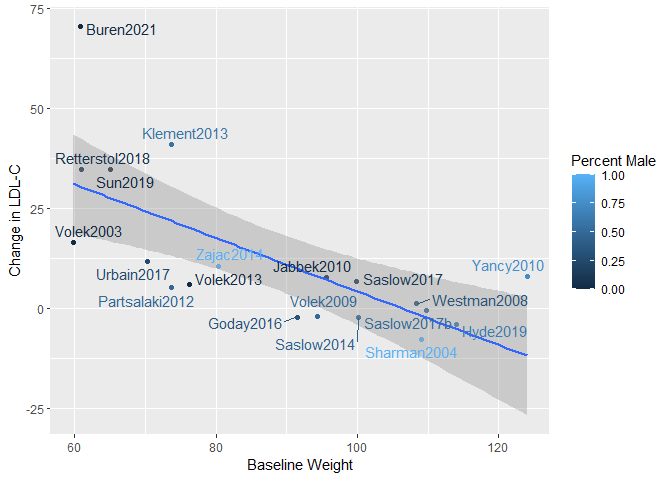
\includegraphics{figures/ldl-change-vs-weight-5.png}

\begin{Shaded}
\begin{Highlighting}[]
\NormalTok{eval.data }\SpecialCharTok{\%\textgreater{}\%}
  \FunctionTok{ggplot}\NormalTok{(}\FunctionTok{aes}\NormalTok{(}\AttributeTok{y=}\StringTok{\textasciigrave{}}\AttributeTok{Change in LDL{-}C}\StringTok{\textasciigrave{}}\NormalTok{,}
             \AttributeTok{x=}\StringTok{\textasciigrave{}}\AttributeTok{Baseline Weight}\StringTok{\textasciigrave{}}\NormalTok{,}
             \AttributeTok{col=}\StringTok{\textasciigrave{}}\AttributeTok{Sex.Group}\StringTok{\textasciigrave{}}\NormalTok{)) }\SpecialCharTok{+}
  \FunctionTok{geom\_point}\NormalTok{() }\SpecialCharTok{+}
  \FunctionTok{geom\_smooth}\NormalTok{(}\AttributeTok{method=}\StringTok{\textquotesingle{}lm\textquotesingle{}}\NormalTok{) }\SpecialCharTok{+}
  \FunctionTok{geom\_text\_repel}\NormalTok{(}\FunctionTok{aes}\NormalTok{(}\AttributeTok{label=}\NormalTok{Study)) }\SpecialCharTok{+}
  \FunctionTok{labs}\NormalTok{(}\AttributeTok{x=}\StringTok{"Baseline Weight"}\NormalTok{)}
\end{Highlighting}
\end{Shaded}

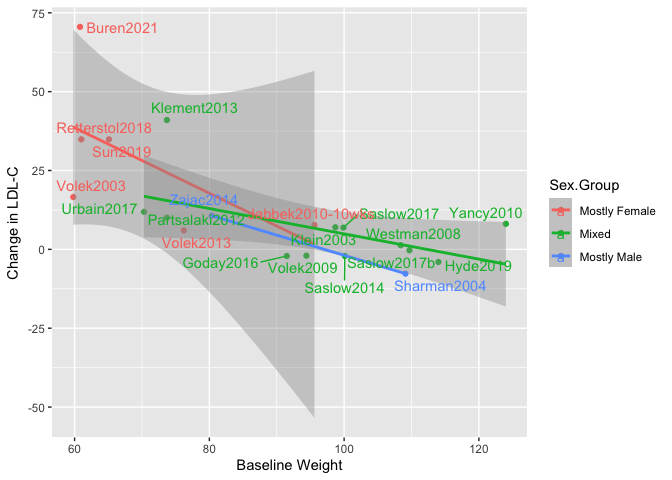
\includegraphics{figures/ldl-change-vs-weight-6.png}

\begin{Shaded}
\begin{Highlighting}[]
\FunctionTok{library}\NormalTok{(broom)}
\FunctionTok{bind\_rows}\NormalTok{(}\StringTok{\textasciigrave{}}\AttributeTok{Baseline}\StringTok{\textasciigrave{}}\OtherTok{=}\FunctionTok{shapiro.test}\NormalTok{(eval.data}\SpecialCharTok{$}\StringTok{\textasciigrave{}}\AttributeTok{Baseline Weight}\StringTok{\textasciigrave{}}\NormalTok{)}\SpecialCharTok{$}\NormalTok{p.value,}
          \StringTok{\textasciigrave{}}\AttributeTok{Change}\StringTok{\textasciigrave{}}\OtherTok{=}\FunctionTok{shapiro.test}\NormalTok{(eval.data}\SpecialCharTok{$}\StringTok{\textasciigrave{}}\AttributeTok{Change in LDL{-}C}\StringTok{\textasciigrave{}}\NormalTok{)}\SpecialCharTok{$}\NormalTok{p.value) }\SpecialCharTok{\%\textgreater{}\%}
  \FunctionTok{kable}\NormalTok{(}\AttributeTok{caption=}\StringTok{"Shapiro Tests for Correlates"}\NormalTok{)}
\end{Highlighting}
\end{Shaded}

\begin{longtable}[]{@{}rr@{}}
\caption{Shapiro Tests for Correlates}\tabularnewline
\toprule
Baseline & Change \\
\midrule
\endfirsthead
\toprule
Baseline & Change \\
\midrule
\endhead
0.216 & 0 \\
\bottomrule
\end{longtable}

\begin{Shaded}
\begin{Highlighting}[]
\FunctionTok{with}\NormalTok{(eval.data, }\FunctionTok{cor.test}\NormalTok{(}\StringTok{\textasciigrave{}}\AttributeTok{Change in LDL{-}C}\StringTok{\textasciigrave{}}\NormalTok{,}\StringTok{\textasciigrave{}}\AttributeTok{Baseline Weight}\StringTok{\textasciigrave{}}\NormalTok{, }\AttributeTok{method=}\StringTok{"spearman"}\NormalTok{)) }\SpecialCharTok{\%\textgreater{}\%}\NormalTok{ tidy }\SpecialCharTok{\%\textgreater{}\%} \FunctionTok{kable}\NormalTok{(}\AttributeTok{caption=}\StringTok{"Correlation between change in LDL{-}C and baseline weight"}\NormalTok{)}
\end{Highlighting}
\end{Shaded}

\begin{longtable}[]{@{}rrrll@{}}
\caption{Correlation between change in LDL-C and baseline
weight}\tabularnewline
\toprule
estimate & statistic & p.value & method & alternative \\
\midrule
\endfirsthead
\toprule
estimate & statistic & p.value & method & alternative \\
\midrule
\endhead
-0.725 & 1966 & 0 & Spearman's rank correlation rho & two.sided \\
\bottomrule
\end{longtable}

\begin{Shaded}
\begin{Highlighting}[]
\FunctionTok{lm}\NormalTok{(}\StringTok{\textasciigrave{}}\AttributeTok{Change in LDL{-}C}\StringTok{\textasciigrave{}}\SpecialCharTok{\textasciitilde{}}\StringTok{\textasciigrave{}}\AttributeTok{Baseline Weight}\StringTok{\textasciigrave{}}\SpecialCharTok{+}\StringTok{\textasciigrave{}}\AttributeTok{Percent Male}\StringTok{\textasciigrave{}}\NormalTok{, }\AttributeTok{data=}\NormalTok{eval.data) }\SpecialCharTok{\%\textgreater{}\%}\NormalTok{ tidy }\SpecialCharTok{\%\textgreater{}\%} \FunctionTok{kable}\NormalTok{(}\AttributeTok{caption=}\StringTok{"Linear model between change in LDL{-}C and baseline weight, including gender"}\NormalTok{)}
\end{Highlighting}
\end{Shaded}

\begin{longtable}[]{@{}lrrrr@{}}
\caption{Linear model between change in LDL-C and baseline weight,
including gender}\tabularnewline
\toprule
term & estimate & std.error & statistic & p.value \\
\midrule
\endfirsthead
\toprule
term & estimate & std.error & statistic & p.value \\
\midrule
\endhead
(Intercept) & 69.286 & 16.562 & 4.183 & 0.001 \\
\texttt{Baseline\ Weight} & -0.627 & 0.208 & -3.013 & 0.008 \\
\texttt{Percent\ Male} & -4.849 & 12.797 & -0.379 & 0.710 \\
\bottomrule
\end{longtable}

\begin{Shaded}
\begin{Highlighting}[]
\NormalTok{ldl.weight.baseline.lm }\OtherTok{\textless{}{-}} \FunctionTok{lm}\NormalTok{(}\StringTok{\textasciigrave{}}\AttributeTok{Change in LDL{-}C}\StringTok{\textasciigrave{}} \SpecialCharTok{\textasciitilde{}} \StringTok{\textasciigrave{}}\AttributeTok{Baseline Weight}\StringTok{\textasciigrave{}} \SpecialCharTok{+} \StringTok{\textasciigrave{}}\AttributeTok{Sex.Group}\StringTok{\textasciigrave{}}\NormalTok{, }\AttributeTok{data =}\NormalTok{ eval.data)}
\NormalTok{ldl.weight.baseline.lm }\SpecialCharTok{\%\textgreater{}\%}\NormalTok{ tidy }\SpecialCharTok{\%\textgreater{}\%}\NormalTok{ kable}
\end{Highlighting}
\end{Shaded}

\begin{longtable}[]{@{}lrrrr@{}}
\toprule
term & estimate & std.error & statistic & p.value \\
\midrule
\endhead
(Intercept) & 65.991 & 16.716 & 3.948 & 0.001 \\
\texttt{Baseline\ Weight} & -0.538 & 0.223 & -2.415 & 0.029 \\
Sex.GroupMixed & -8.305 & 9.667 & -0.859 & 0.404 \\
Sex.GroupMostly Male & -13.512 & 13.489 & -1.002 & 0.332 \\
\bottomrule
\end{longtable}

\begin{Shaded}
\begin{Highlighting}[]
\NormalTok{ldl.bmi.baseline.lm }\OtherTok{\textless{}{-}} \FunctionTok{lm}\NormalTok{(}\StringTok{\textasciigrave{}}\AttributeTok{Change in LDL{-}C}\StringTok{\textasciigrave{}} \SpecialCharTok{\textasciitilde{}} \StringTok{\textasciigrave{}}\AttributeTok{Baseline BMI}\StringTok{\textasciigrave{}} \SpecialCharTok{+} \StringTok{\textasciigrave{}}\AttributeTok{Sex.Group}\StringTok{\textasciigrave{}}\NormalTok{, }\AttributeTok{data =}\NormalTok{ eval.data)}
\NormalTok{ldl.bmi.baseline.lm }\SpecialCharTok{\%\textgreater{}\%}\NormalTok{ tidy }\SpecialCharTok{\%\textgreater{}\%}\NormalTok{ kable}
\end{Highlighting}
\end{Shaded}

\begin{longtable}[]{@{}lrrrr@{}}
\toprule
term & estimate & std.error & statistic & p.value \\
\midrule
\endhead
(Intercept) & 55.84 & 13.636 & 4.09 & 0.003 \\
\texttt{Baseline\ BMI} & -1.13 & 0.489 & -2.31 & 0.050 \\
Sex.GroupMixed & -14.57 & 5.951 & -2.45 & 0.040 \\
Sex.GroupMostly Male & -17.01 & 8.376 & -2.03 & 0.077 \\
\bottomrule
\end{longtable}

\begin{Shaded}
\begin{Highlighting}[]
\NormalTok{ldl.weight.baseline.aov }\OtherTok{\textless{}{-}} \FunctionTok{aov}\NormalTok{(}\StringTok{\textasciigrave{}}\AttributeTok{Change in LDL{-}C}\StringTok{\textasciigrave{}} \SpecialCharTok{\textasciitilde{}} \StringTok{\textasciigrave{}}\AttributeTok{Baseline Weight}\StringTok{\textasciigrave{}} \SpecialCharTok{+} \StringTok{\textasciigrave{}}\AttributeTok{Sex.Group}\StringTok{\textasciigrave{}}\NormalTok{, }\AttributeTok{data =}\NormalTok{ eval.data)}
\NormalTok{ldl.weight.baseline.aov }\SpecialCharTok{\%\textgreater{}\%}\NormalTok{ tidy }\SpecialCharTok{\%\textgreater{}\%}\NormalTok{ kable}
\end{Highlighting}
\end{Shaded}

\begin{longtable}[]{@{}lrrrrr@{}}
\toprule
term & df & sumsq & meansq & statistic & p.value \\
\midrule
\endhead
\texttt{Baseline\ Weight} & 1 & 3319 & 3319 & 14.655 & 0.002 \\
Sex.Group & 2 & 259 & 130 & 0.572 & 0.576 \\
Residuals & 15 & 3397 & 226 & NA & NA \\
\bottomrule
\end{longtable}

\begin{Shaded}
\begin{Highlighting}[]
\NormalTok{ldl.bmi.baseline.aov }\OtherTok{\textless{}{-}} \FunctionTok{aov}\NormalTok{(}\StringTok{\textasciigrave{}}\AttributeTok{Change in LDL{-}C}\StringTok{\textasciigrave{}} \SpecialCharTok{\textasciitilde{}} \StringTok{\textasciigrave{}}\AttributeTok{Baseline BMI}\StringTok{\textasciigrave{}} \SpecialCharTok{+} \StringTok{\textasciigrave{}}\AttributeTok{Sex.Group}\StringTok{\textasciigrave{}}\NormalTok{, }\AttributeTok{data =}\NormalTok{ eval.data)}
\NormalTok{ldl.bmi.baseline.aov }\SpecialCharTok{\%\textgreater{}\%}\NormalTok{ tidy }\SpecialCharTok{\%\textgreater{}\%}\NormalTok{ kable}
\end{Highlighting}
\end{Shaded}

\begin{longtable}[]{@{}lrrrrr@{}}
\toprule
term & df & sumsq & meansq & statistic & p.value \\
\midrule
\endhead
\texttt{Baseline\ BMI} & 1 & 965 & 965.0 & 18.51 & 0.003 \\
Sex.Group & 2 & 411 & 205.3 & 3.94 & 0.065 \\
Residuals & 8 & 417 & 52.1 & NA & NA \\
\bottomrule
\end{longtable}

\begin{Shaded}
\begin{Highlighting}[]
\NormalTok{ldl.bmi2.baseline.aov }\OtherTok{\textless{}{-}} \FunctionTok{aov}\NormalTok{(}\StringTok{\textasciigrave{}}\AttributeTok{Change in LDL{-}C}\StringTok{\textasciigrave{}} \SpecialCharTok{\textasciitilde{}} \StringTok{\textasciigrave{}}\AttributeTok{Baseline BMI}\StringTok{\textasciigrave{}}\SpecialCharTok{*}\StringTok{\textasciigrave{}}\AttributeTok{Sex.Group}\StringTok{\textasciigrave{}}\NormalTok{, }\AttributeTok{data =}\NormalTok{ eval.data)}
\NormalTok{ldl.bmi2.baseline.aov }\SpecialCharTok{\%\textgreater{}\%}\NormalTok{ tidy }\SpecialCharTok{\%\textgreater{}\%}\NormalTok{ kable}
\end{Highlighting}
\end{Shaded}

\begin{longtable}[]{@{}lrrrrr@{}}
\toprule
term & df & sumsq & meansq & statistic & p.value \\
\midrule
\endhead
\texttt{Baseline\ BMI} & 1 & 965 & 965.0 & 32.26 & 0.001 \\
Sex.Group & 2 & 411 & 205.3 & 6.86 & 0.022 \\
\texttt{Baseline\ BMI}:Sex.Group & 1 & 208 & 207.7 & 6.94 & 0.034 \\
Residuals & 7 & 209 & 29.9 & NA & NA \\
\bottomrule
\end{longtable}

\begin{Shaded}
\begin{Highlighting}[]
\NormalTok{ldl.weight.baseline.aov }\OtherTok{\textless{}{-}} \FunctionTok{aov}\NormalTok{(}\StringTok{\textasciigrave{}}\AttributeTok{Change in LDL{-}C}\StringTok{\textasciigrave{}} \SpecialCharTok{\textasciitilde{}} \StringTok{\textasciigrave{}}\AttributeTok{Baseline Weight}\StringTok{\textasciigrave{}}\NormalTok{, }\AttributeTok{data =}\NormalTok{ eval.data)}
\NormalTok{ldl.weight.baseline.aov }\SpecialCharTok{\%\textgreater{}\%}\NormalTok{ tidy }\SpecialCharTok{\%\textgreater{}\%}\NormalTok{ kable}
\end{Highlighting}
\end{Shaded}

\begin{longtable}[]{@{}lrrrrr@{}}
\toprule
term & df & sumsq & meansq & statistic & p.value \\
\midrule
\endhead
\texttt{Baseline\ Weight} & 1 & 3319 & 3319 & 15.4 & 0.001 \\
Residuals & 17 & 3657 & 215 & NA & NA \\
\bottomrule
\end{longtable}

\hypertarget{relative-to-weight-loss}{%
\subsection{Relative to Weight Loss}\label{relative-to-weight-loss}}

\begin{Shaded}
\begin{Highlighting}[]
\FunctionTok{library}\NormalTok{(ggplot2)}

\NormalTok{eval.data }\SpecialCharTok{\%\textgreater{}\%}
  \FunctionTok{ggplot}\NormalTok{(}\FunctionTok{aes}\NormalTok{(}\AttributeTok{y=}\StringTok{\textasciigrave{}}\AttributeTok{Change in LDL{-}C}\StringTok{\textasciigrave{}}\NormalTok{,}
             \AttributeTok{x=}\NormalTok{Pct.Wt.Change)) }\SpecialCharTok{+}
  \FunctionTok{geom\_point}\NormalTok{() }\SpecialCharTok{+}
  \FunctionTok{geom\_smooth}\NormalTok{(}\AttributeTok{method=}\StringTok{\textquotesingle{}lm\textquotesingle{}}\NormalTok{) }\SpecialCharTok{+}
  \FunctionTok{geom\_text\_repel}\NormalTok{(}\FunctionTok{aes}\NormalTok{(}\AttributeTok{label=}\NormalTok{Study)) }\SpecialCharTok{+}
  \FunctionTok{labs}\NormalTok{(}\AttributeTok{x=}\StringTok{"Weight Change (\%)"}\NormalTok{)}
\end{Highlighting}
\end{Shaded}

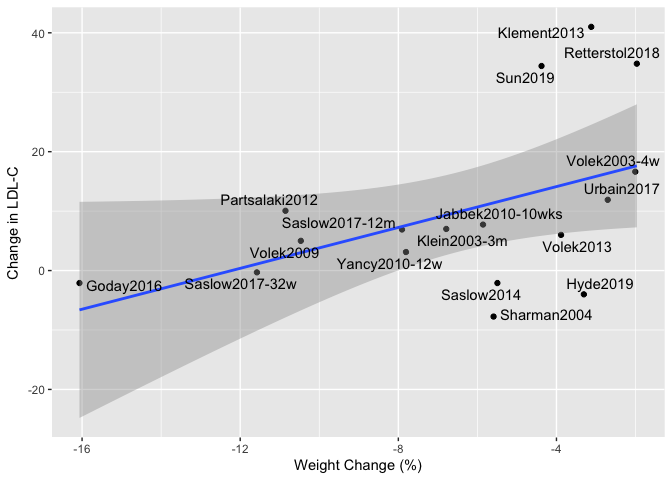
\includegraphics{figures/ldl-change-vs-weight-change-1.png}

\begin{Shaded}
\begin{Highlighting}[]
\NormalTok{eval.data }\SpecialCharTok{\%\textgreater{}\%}
  \FunctionTok{ggplot}\NormalTok{(}\FunctionTok{aes}\NormalTok{(}\AttributeTok{y=}\StringTok{\textasciigrave{}}\AttributeTok{Change in LDL{-}C}\StringTok{\textasciigrave{}}\NormalTok{,}
             \AttributeTok{x=}\StringTok{\textasciigrave{}}\AttributeTok{BMI Change}\StringTok{\textasciigrave{}}\NormalTok{)) }\SpecialCharTok{+}
  \FunctionTok{geom\_point}\NormalTok{() }\SpecialCharTok{+}
  \FunctionTok{geom\_smooth}\NormalTok{(}\AttributeTok{method=}\StringTok{\textquotesingle{}lm\textquotesingle{}}\NormalTok{) }\SpecialCharTok{+}
  \FunctionTok{geom\_text\_repel}\NormalTok{(}\FunctionTok{aes}\NormalTok{(}\AttributeTok{label=}\NormalTok{Study)) }\SpecialCharTok{+}
  \FunctionTok{labs}\NormalTok{(}\AttributeTok{x=}\StringTok{"BMI Change"}\NormalTok{)}
\end{Highlighting}
\end{Shaded}

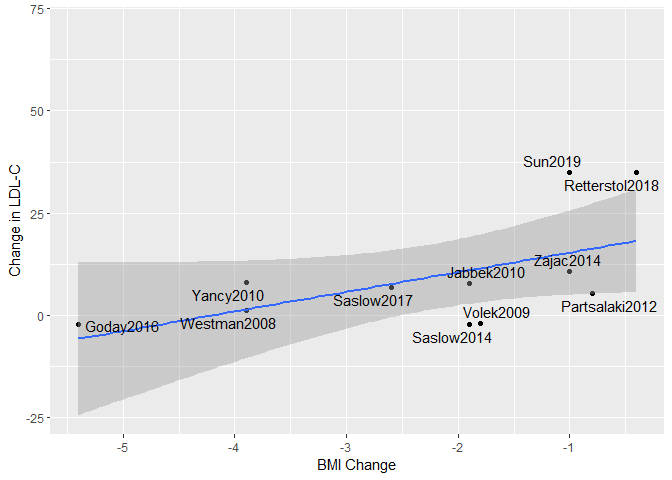
\includegraphics{figures/ldl-change-vs-weight-change-2.png}

\begin{Shaded}
\begin{Highlighting}[]
\NormalTok{eval.data }\SpecialCharTok{\%\textgreater{}\%}
  \FunctionTok{ggplot}\NormalTok{(}\FunctionTok{aes}\NormalTok{(}\AttributeTok{y=}\StringTok{\textasciigrave{}}\AttributeTok{Change in LDL{-}C}\StringTok{\textasciigrave{}}\NormalTok{,}
             \AttributeTok{x=}\StringTok{\textasciigrave{}}\AttributeTok{PCT.BMI.Change}\StringTok{\textasciigrave{}}\NormalTok{)) }\SpecialCharTok{+}
  \FunctionTok{geom\_point}\NormalTok{() }\SpecialCharTok{+}
  \FunctionTok{geom\_smooth}\NormalTok{(}\AttributeTok{method=}\StringTok{\textquotesingle{}lm\textquotesingle{}}\NormalTok{) }\SpecialCharTok{+}
  \FunctionTok{geom\_text\_repel}\NormalTok{(}\FunctionTok{aes}\NormalTok{(}\AttributeTok{label=}\NormalTok{Study)) }\SpecialCharTok{+}
  \FunctionTok{labs}\NormalTok{(}\AttributeTok{x=}\StringTok{"\% BMI Change"}\NormalTok{)}
\end{Highlighting}
\end{Shaded}

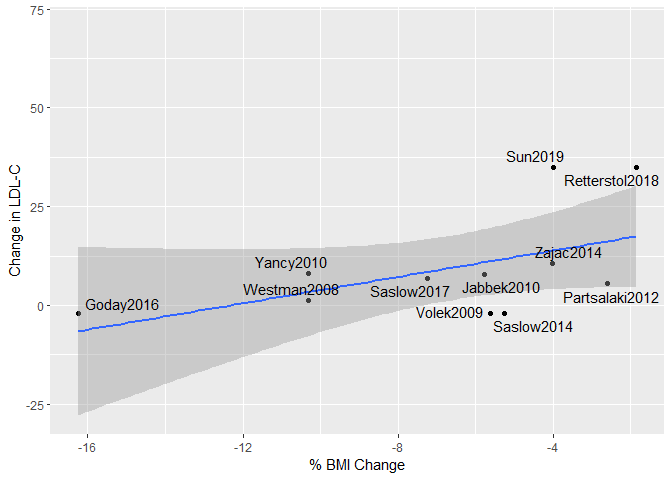
\includegraphics{figures/ldl-change-vs-weight-change-3.png}

\begin{Shaded}
\begin{Highlighting}[]
\NormalTok{eval.data }\SpecialCharTok{\%\textgreater{}\%}
  \FunctionTok{ggplot}\NormalTok{(}\FunctionTok{aes}\NormalTok{(}\AttributeTok{y=}\StringTok{\textasciigrave{}}\AttributeTok{Change in LDL{-}C}\StringTok{\textasciigrave{}}\NormalTok{,}
             \AttributeTok{x=}\NormalTok{Pct.Wt.Change,}
             \AttributeTok{col=}\StringTok{\textasciigrave{}}\AttributeTok{Percent Male}\StringTok{\textasciigrave{}}\NormalTok{)) }\SpecialCharTok{+}
  \FunctionTok{geom\_point}\NormalTok{() }\SpecialCharTok{+}
  \FunctionTok{geom\_smooth}\NormalTok{(}\AttributeTok{method=}\StringTok{\textquotesingle{}lm\textquotesingle{}}\NormalTok{) }\SpecialCharTok{+}
  \FunctionTok{geom\_text\_repel}\NormalTok{(}\FunctionTok{aes}\NormalTok{(}\AttributeTok{label=}\NormalTok{Study)) }\SpecialCharTok{+}
  \FunctionTok{labs}\NormalTok{(}\AttributeTok{x=}\StringTok{"Weight Change (\%)"}\NormalTok{)}
\end{Highlighting}
\end{Shaded}

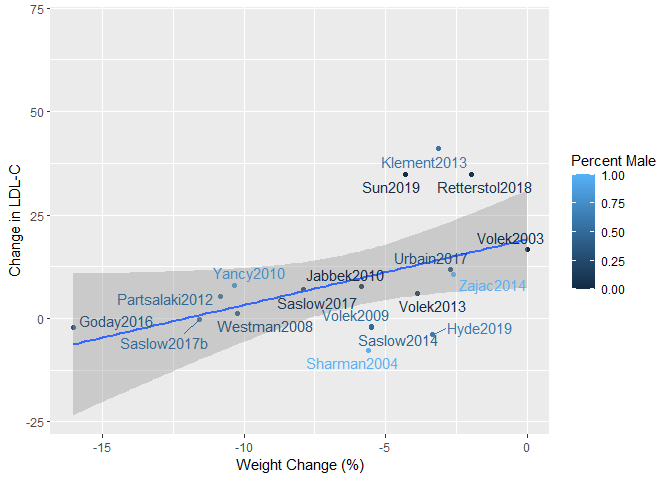
\includegraphics{figures/ldl-change-vs-weight-change-4.png}

\begin{Shaded}
\begin{Highlighting}[]
\FunctionTok{library}\NormalTok{(broom)}
\FunctionTok{bind\_rows}\NormalTok{(}\StringTok{\textasciigrave{}}\AttributeTok{Weight Change}\StringTok{\textasciigrave{}}\OtherTok{=}\FunctionTok{shapiro.test}\NormalTok{(eval.data}\SpecialCharTok{$}\NormalTok{Pct.Wt.Change)}\SpecialCharTok{$}\NormalTok{p.value,}
          \StringTok{\textasciigrave{}}\AttributeTok{LDL Change}\StringTok{\textasciigrave{}}\OtherTok{=}\FunctionTok{shapiro.test}\NormalTok{(eval.data}\SpecialCharTok{$}\StringTok{\textasciigrave{}}\AttributeTok{Change in LDL{-}C}\StringTok{\textasciigrave{}}\NormalTok{)}\SpecialCharTok{$}\NormalTok{p.value) }\SpecialCharTok{\%\textgreater{}\%}
  \FunctionTok{kable}\NormalTok{(}\AttributeTok{caption=}\StringTok{"Shapiro Tests for Correlates"}\NormalTok{)}
\end{Highlighting}
\end{Shaded}

\begin{longtable}[]{@{}rr@{}}
\caption{Shapiro Tests for Correlates}\tabularnewline
\toprule
Weight Change & LDL Change \\
\midrule
\endfirsthead
\toprule
Weight Change & LDL Change \\
\midrule
\endhead
0.199 & 0 \\
\bottomrule
\end{longtable}

\begin{Shaded}
\begin{Highlighting}[]
\FunctionTok{with}\NormalTok{(eval.data, }\FunctionTok{cor.test}\NormalTok{(}\StringTok{\textasciigrave{}}\AttributeTok{Change in LDL{-}C}\StringTok{\textasciigrave{}}\NormalTok{,Pct.Wt.Change, }\AttributeTok{method=}\StringTok{"spearman"}\NormalTok{)) }\SpecialCharTok{\%\textgreater{}\%}\NormalTok{ tidy }\SpecialCharTok{\%\textgreater{}\%} \FunctionTok{kable}\NormalTok{(}\AttributeTok{caption=}\StringTok{"Correlation between change in LDL{-}C and weight change"}\NormalTok{)}
\end{Highlighting}
\end{Shaded}

\begin{longtable}[]{@{}rrrll@{}}
\caption{Correlation between change in LDL-C and weight
change}\tabularnewline
\toprule
estimate & statistic & p.value & method & alternative \\
\midrule
\endfirsthead
\toprule
estimate & statistic & p.value & method & alternative \\
\midrule
\endhead
0.538 & 448 & 0.023 & Spearman's rank correlation rho & two.sided \\
\bottomrule
\end{longtable}

\begin{Shaded}
\begin{Highlighting}[]
\NormalTok{ldl.weight.change.lm }\OtherTok{\textless{}{-}} \FunctionTok{lm}\NormalTok{(}\StringTok{\textasciigrave{}}\AttributeTok{Change in LDL{-}C}\StringTok{\textasciigrave{}} \SpecialCharTok{\textasciitilde{}} \StringTok{\textasciigrave{}}\AttributeTok{Pct.Wt.Change}\StringTok{\textasciigrave{}} \SpecialCharTok{+} \StringTok{\textasciigrave{}}\AttributeTok{Sex.Group}\StringTok{\textasciigrave{}}\NormalTok{, }\AttributeTok{data =}\NormalTok{ eval.data)}
\NormalTok{ldl.weight.change.lm }\SpecialCharTok{\%\textgreater{}\%}\NormalTok{ tidy }\SpecialCharTok{\%\textgreater{}\%}\NormalTok{ kable}
\end{Highlighting}
\end{Shaded}

\begin{longtable}[]{@{}lrrrr@{}}
\toprule
term & estimate & std.error & statistic & p.value \\
\midrule
\endhead
(Intercept) & 24.22 & 6.314 & 3.84 & 0.002 \\
Pct.Wt.Change & 1.31 & 0.878 & 1.49 & 0.158 \\
Sex.GroupMixed & -8.02 & 7.977 & -1.00 & 0.332 \\
Sex.GroupMostly Male & -17.37 & 10.604 & -1.64 & 0.124 \\
\bottomrule
\end{longtable}

\begin{Shaded}
\begin{Highlighting}[]
\NormalTok{ldl.bmi.change.lm }\OtherTok{\textless{}{-}} \FunctionTok{lm}\NormalTok{(}\StringTok{\textasciigrave{}}\AttributeTok{Change in LDL{-}C}\StringTok{\textasciigrave{}} \SpecialCharTok{\textasciitilde{}} \StringTok{\textasciigrave{}}\AttributeTok{BMI Change}\StringTok{\textasciigrave{}} \SpecialCharTok{+} \StringTok{\textasciigrave{}}\AttributeTok{Sex.Group}\StringTok{\textasciigrave{}}\NormalTok{, }\AttributeTok{data =}\NormalTok{ eval.data)}
\NormalTok{ldl.bmi.change.lm }\SpecialCharTok{\%\textgreater{}\%}\NormalTok{ tidy }\SpecialCharTok{\%\textgreater{}\%}\NormalTok{ kable}
\end{Highlighting}
\end{Shaded}

\begin{longtable}[]{@{}lrrrr@{}}
\toprule
term & estimate & std.error & statistic & p.value \\
\midrule
\endhead
(Intercept) & 27.67 & 5.76 & 4.801 & 0.002 \\
\texttt{BMI\ Change} & 1.66 & 2.25 & 0.739 & 0.484 \\
Sex.GroupMixed & -20.64 & 7.42 & -2.781 & 0.027 \\
Sex.GroupMostly Male & -15.33 & 10.41 & -1.472 & 0.185 \\
\bottomrule
\end{longtable}

\begin{Shaded}
\begin{Highlighting}[]
\NormalTok{ldl.pctbmi.change.lm }\OtherTok{\textless{}{-}} \FunctionTok{lm}\NormalTok{(}\StringTok{\textasciigrave{}}\AttributeTok{Change in LDL{-}C}\StringTok{\textasciigrave{}} \SpecialCharTok{\textasciitilde{}} \StringTok{\textasciigrave{}}\AttributeTok{PCT.BMI.Change}\StringTok{\textasciigrave{}} \SpecialCharTok{+} \StringTok{\textasciigrave{}}\AttributeTok{Sex.Group}\StringTok{\textasciigrave{}}\NormalTok{, }\AttributeTok{data =}\NormalTok{ eval.data)}
\NormalTok{ldl.pctbmi.change.lm }\SpecialCharTok{\%\textgreater{}\%}\NormalTok{ tidy }\SpecialCharTok{\%\textgreater{}\%}\NormalTok{ kable}
\end{Highlighting}
\end{Shaded}

\begin{longtable}[]{@{}lrrrr@{}}
\toprule
term & estimate & std.error & statistic & p.value \\
\midrule
\endhead
(Intercept) & 28.078 & 6.051 & 4.640 & 0.002 \\
PCT.BMI.Change & 0.578 & 0.794 & 0.728 & 0.490 \\
Sex.GroupMixed & -21.108 & 7.123 & -2.963 & 0.021 \\
Sex.GroupMostly Male & -15.077 & 10.423 & -1.447 & 0.191 \\
\bottomrule
\end{longtable}

\begin{Shaded}
\begin{Highlighting}[]
\NormalTok{ldl.weight.change.aov }\OtherTok{\textless{}{-}} \FunctionTok{aov}\NormalTok{(}\StringTok{\textasciigrave{}}\AttributeTok{Change in LDL{-}C}\StringTok{\textasciigrave{}} \SpecialCharTok{\textasciitilde{}} \StringTok{\textasciigrave{}}\AttributeTok{Pct.Wt.Change}\StringTok{\textasciigrave{}} \SpecialCharTok{+} \StringTok{\textasciigrave{}}\AttributeTok{Sex.Group}\StringTok{\textasciigrave{}}\NormalTok{, }\AttributeTok{data =}\NormalTok{ eval.data)}
\NormalTok{ldl.weight.change.aov }\SpecialCharTok{\%\textgreater{}\%}\NormalTok{ tidy }\SpecialCharTok{\%\textgreater{}\%}\NormalTok{ kable}
\end{Highlighting}
\end{Shaded}

\begin{longtable}[]{@{}lrrrrr@{}}
\toprule
term & df & sumsq & meansq & statistic & p.value \\
\midrule
\endhead
Pct.Wt.Change & 1 & 735 & 735 & 4.60 & 0.050 \\
Sex.Group & 2 & 449 & 225 & 1.40 & 0.278 \\
Residuals & 14 & 2237 & 160 & NA & NA \\
\bottomrule
\end{longtable}

\begin{Shaded}
\begin{Highlighting}[]
\NormalTok{ldl.bmi.change.aov }\OtherTok{\textless{}{-}} \FunctionTok{aov}\NormalTok{(}\StringTok{\textasciigrave{}}\AttributeTok{Change in LDL{-}C}\StringTok{\textasciigrave{}} \SpecialCharTok{\textasciitilde{}} \StringTok{\textasciigrave{}}\AttributeTok{BMI Change}\StringTok{\textasciigrave{}} \SpecialCharTok{+} \StringTok{\textasciigrave{}}\AttributeTok{Sex.Group}\StringTok{\textasciigrave{}}\NormalTok{, }\AttributeTok{data =}\NormalTok{ eval.data)}
\NormalTok{ldl.bmi.change.aov }\SpecialCharTok{\%\textgreater{}\%}\NormalTok{ tidy }\SpecialCharTok{\%\textgreater{}\%}\NormalTok{ kable}
\end{Highlighting}
\end{Shaded}

\begin{longtable}[]{@{}lrrrrr@{}}
\toprule
term & df & sumsq & meansq & statistic & p.value \\
\midrule
\endhead
\texttt{BMI\ Change} & 1 & 564 & 563.8 & 6.93 & 0.034 \\
Sex.Group & 2 & 654 & 327.1 & 4.03 & 0.069 \\
Residuals & 7 & 569 & 81.3 & NA & NA \\
\bottomrule
\end{longtable}

\begin{Shaded}
\begin{Highlighting}[]
\NormalTok{ldl.pctbmi.change.aov }\OtherTok{\textless{}{-}} \FunctionTok{aov}\NormalTok{(}\StringTok{\textasciigrave{}}\AttributeTok{Change in LDL{-}C}\StringTok{\textasciigrave{}} \SpecialCharTok{\textasciitilde{}} \StringTok{\textasciigrave{}}\AttributeTok{PCT.BMI.Change}\StringTok{\textasciigrave{}} \SpecialCharTok{+} \StringTok{\textasciigrave{}}\AttributeTok{Sex.Group}\StringTok{\textasciigrave{}}\NormalTok{, }\AttributeTok{data =}\NormalTok{ eval.data)}
\NormalTok{ldl.pctbmi.change.aov }\SpecialCharTok{\%\textgreater{}\%}\NormalTok{ tidy }\SpecialCharTok{\%\textgreater{}\%}\NormalTok{ kable}
\end{Highlighting}
\end{Shaded}

\begin{longtable}[]{@{}lrrrrr@{}}
\toprule
term & df & sumsq & meansq & statistic & p.value \\
\midrule
\endhead
PCT.BMI.Change & 1 & 490 & 490.1 & 6.02 & 0.044 \\
Sex.Group & 2 & 727 & 363.4 & 4.46 & 0.056 \\
Residuals & 7 & 570 & 81.5 & NA & NA \\
\bottomrule
\end{longtable}

\begin{Shaded}
\begin{Highlighting}[]
\NormalTok{ldl.weight.change.aov }\OtherTok{\textless{}{-}} \FunctionTok{aov}\NormalTok{(}\StringTok{\textasciigrave{}}\AttributeTok{Change in LDL{-}C}\StringTok{\textasciigrave{}} \SpecialCharTok{\textasciitilde{}} \StringTok{\textasciigrave{}}\AttributeTok{Pct.Wt.Change}\StringTok{\textasciigrave{}}\NormalTok{, }\AttributeTok{data =}\NormalTok{ eval.data)}
\NormalTok{ldl.weight.change.aov }\SpecialCharTok{\%\textgreater{}\%}\NormalTok{ tidy }\SpecialCharTok{\%\textgreater{}\%}\NormalTok{ kable}
\end{Highlighting}
\end{Shaded}

\begin{longtable}[]{@{}lrrrrr@{}}
\toprule
term & df & sumsq & meansq & statistic & p.value \\
\midrule
\endhead
Pct.Wt.Change & 1 & 735 & 735 & 4.38 & 0.053 \\
Residuals & 16 & 2686 & 168 & NA & NA \\
\bottomrule
\end{longtable}

\hypertarget{relative-to-baseline-ldl-c}{%
\subsection{Relative to Baseline
LDL-C}\label{relative-to-baseline-ldl-c}}

\begin{Shaded}
\begin{Highlighting}[]
\FunctionTok{library}\NormalTok{(ggplot2)}
\NormalTok{eval.data }\SpecialCharTok{\%\textgreater{}\%}
  \FunctionTok{ggplot}\NormalTok{(}\FunctionTok{aes}\NormalTok{(}\AttributeTok{y=}\StringTok{\textasciigrave{}}\AttributeTok{Change in LDL{-}C}\StringTok{\textasciigrave{}}\NormalTok{,}
             \AttributeTok{x=}\StringTok{\textasciigrave{}}\AttributeTok{Baseline LDL}\StringTok{\textasciigrave{}}\NormalTok{)) }\SpecialCharTok{+}
  \FunctionTok{geom\_point}\NormalTok{() }\SpecialCharTok{+}
  \FunctionTok{geom\_smooth}\NormalTok{(}\AttributeTok{method=}\StringTok{\textquotesingle{}lm\textquotesingle{}}\NormalTok{) }\SpecialCharTok{+}
  \FunctionTok{geom\_text\_repel}\NormalTok{(}\FunctionTok{aes}\NormalTok{(}\AttributeTok{label=}\NormalTok{Study)) }\SpecialCharTok{+}
  \FunctionTok{labs}\NormalTok{(}\AttributeTok{x=}\StringTok{"Baseline LDL{-}C"}\NormalTok{)}
\end{Highlighting}
\end{Shaded}

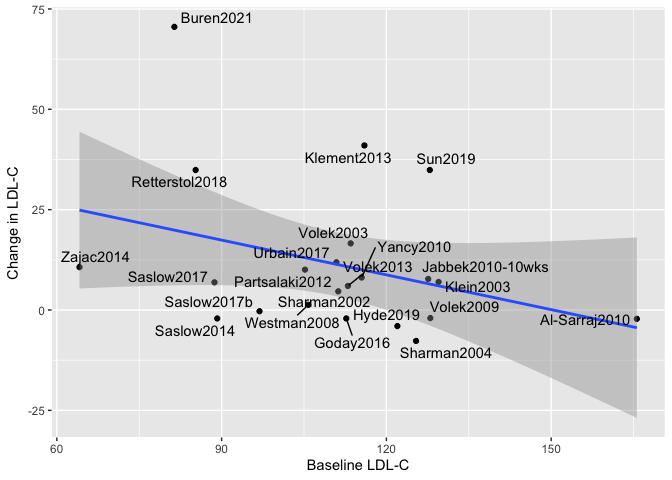
\includegraphics{figures/ldl-change-vs-baseline-1.png}

\begin{Shaded}
\begin{Highlighting}[]
\NormalTok{eval.data }\SpecialCharTok{\%\textgreater{}\%}
  \FunctionTok{ggplot}\NormalTok{(}\FunctionTok{aes}\NormalTok{(}\AttributeTok{y=}\StringTok{\textasciigrave{}}\AttributeTok{Change in LDL{-}C}\StringTok{\textasciigrave{}}\NormalTok{,}
             \AttributeTok{x=}\StringTok{\textasciigrave{}}\AttributeTok{Baseline LDL}\StringTok{\textasciigrave{}}\NormalTok{,}
             \AttributeTok{col=}\StringTok{\textasciigrave{}}\AttributeTok{Percent Male}\StringTok{\textasciigrave{}}\NormalTok{)) }\SpecialCharTok{+}
  \FunctionTok{geom\_point}\NormalTok{() }\SpecialCharTok{+}
  \FunctionTok{geom\_smooth}\NormalTok{(}\AttributeTok{method=}\StringTok{\textquotesingle{}lm\textquotesingle{}}\NormalTok{) }\SpecialCharTok{+}
  \FunctionTok{geom\_text\_repel}\NormalTok{(}\FunctionTok{aes}\NormalTok{(}\AttributeTok{label=}\NormalTok{Study)) }\SpecialCharTok{+}
  \FunctionTok{labs}\NormalTok{(}\AttributeTok{x=}\StringTok{"Baseline LDL{-}C"}\NormalTok{)}
\end{Highlighting}
\end{Shaded}

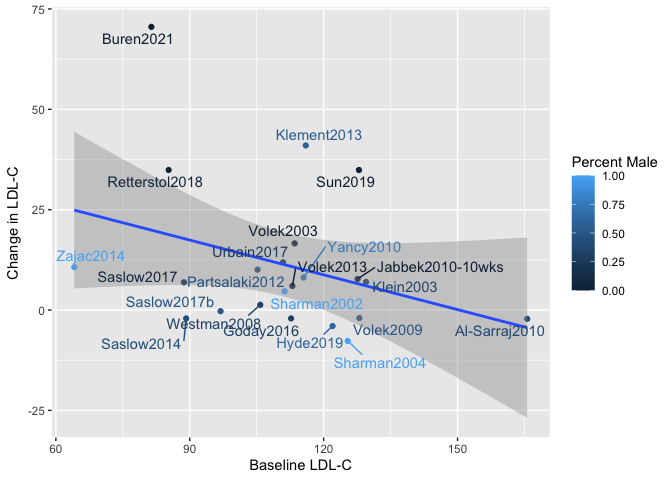
\includegraphics{figures/ldl-change-vs-baseline-2.png}

\begin{Shaded}
\begin{Highlighting}[]
\NormalTok{eval.data }\SpecialCharTok{\%\textgreater{}\%}
  \FunctionTok{ggplot}\NormalTok{(}\FunctionTok{aes}\NormalTok{(}\AttributeTok{y=}\StringTok{\textasciigrave{}}\AttributeTok{Change in LDL{-}C}\StringTok{\textasciigrave{}}\NormalTok{,}
             \AttributeTok{x=}\StringTok{\textasciigrave{}}\AttributeTok{Baseline LDL}\StringTok{\textasciigrave{}}\NormalTok{,}
             \AttributeTok{col=}\StringTok{\textasciigrave{}}\AttributeTok{Sex.Group}\StringTok{\textasciigrave{}}\NormalTok{)) }\SpecialCharTok{+}
  \FunctionTok{geom\_point}\NormalTok{() }\SpecialCharTok{+}
  \FunctionTok{geom\_smooth}\NormalTok{(}\AttributeTok{method=}\StringTok{\textquotesingle{}lm\textquotesingle{}}\NormalTok{) }\SpecialCharTok{+}
  \FunctionTok{geom\_text\_repel}\NormalTok{(}\FunctionTok{aes}\NormalTok{(}\AttributeTok{label=}\NormalTok{Study)) }\SpecialCharTok{+}
  \FunctionTok{labs}\NormalTok{(}\AttributeTok{x=}\StringTok{"Baseline LDL{-}C"}\NormalTok{)}
\end{Highlighting}
\end{Shaded}

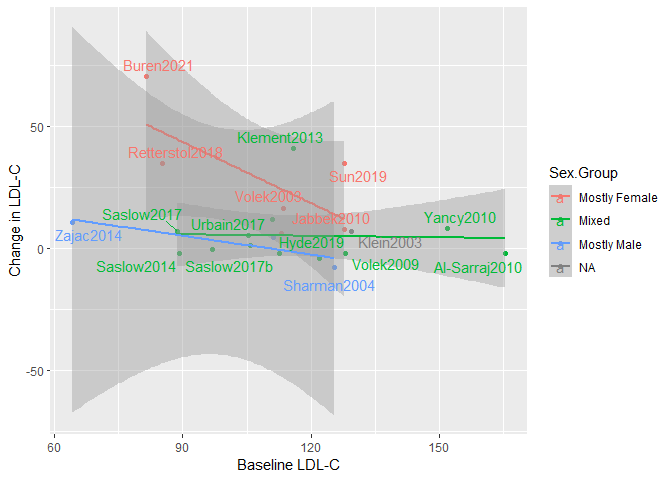
\includegraphics{figures/ldl-change-vs-baseline-3.png}

\begin{Shaded}
\begin{Highlighting}[]
\FunctionTok{library}\NormalTok{(broom)}
\FunctionTok{bind\_rows}\NormalTok{(}\StringTok{\textasciigrave{}}\AttributeTok{Baseline}\StringTok{\textasciigrave{}}\OtherTok{=}\FunctionTok{shapiro.test}\NormalTok{(eval.data}\SpecialCharTok{$}\StringTok{\textasciigrave{}}\AttributeTok{Baseline LDL}\StringTok{\textasciigrave{}}\NormalTok{)}\SpecialCharTok{$}\NormalTok{p.value,}
          \StringTok{\textasciigrave{}}\AttributeTok{Change}\StringTok{\textasciigrave{}}\OtherTok{=}\FunctionTok{shapiro.test}\NormalTok{(eval.data}\SpecialCharTok{$}\StringTok{\textasciigrave{}}\AttributeTok{Change in LDL{-}C}\StringTok{\textasciigrave{}}\NormalTok{)}\SpecialCharTok{$}\NormalTok{p.value) }\SpecialCharTok{\%\textgreater{}\%}
  \FunctionTok{kable}\NormalTok{(}\AttributeTok{caption=}\StringTok{"Shapiro Tests for Correlates"}\NormalTok{)}
\end{Highlighting}
\end{Shaded}

\begin{longtable}[]{@{}rr@{}}
\caption{Shapiro Tests for Correlates}\tabularnewline
\toprule
Baseline & Change \\
\midrule
\endfirsthead
\toprule
Baseline & Change \\
\midrule
\endhead
0.703 & 0 \\
\bottomrule
\end{longtable}

\begin{Shaded}
\begin{Highlighting}[]
\FunctionTok{with}\NormalTok{(eval.data, }\FunctionTok{cor.test}\NormalTok{(}\StringTok{\textasciigrave{}}\AttributeTok{Change in LDL{-}C}\StringTok{\textasciigrave{}}\NormalTok{,}\StringTok{\textasciigrave{}}\AttributeTok{Baseline LDL}\StringTok{\textasciigrave{}}\NormalTok{, }\AttributeTok{method=}\StringTok{"spearman"}\NormalTok{)) }\SpecialCharTok{\%\textgreater{}\%}\NormalTok{ tidy }\SpecialCharTok{\%\textgreater{}\%} \FunctionTok{kable}\NormalTok{(}\AttributeTok{caption=}\StringTok{"Correlation between baseline and change in LDL{-}C"}\NormalTok{)}
\end{Highlighting}
\end{Shaded}

\begin{longtable}[]{@{}rrrll@{}}
\caption{Correlation between baseline and change in
LDL-C}\tabularnewline
\toprule
estimate & statistic & p.value & method & alternative \\
\midrule
\endfirsthead
\toprule
estimate & statistic & p.value & method & alternative \\
\midrule
\endhead
-0.269 & 1954 & 0.238 & Spearman's rank correlation rho & two.sided \\
\bottomrule
\end{longtable}

\begin{Shaded}
\begin{Highlighting}[]
\NormalTok{ldl.baseline.lm }\OtherTok{\textless{}{-}} \FunctionTok{lm}\NormalTok{(}\StringTok{\textasciigrave{}}\AttributeTok{Change in LDL{-}C}\StringTok{\textasciigrave{}} \SpecialCharTok{\textasciitilde{}} \StringTok{\textasciigrave{}}\AttributeTok{Baseline LDL}\StringTok{\textasciigrave{}} \SpecialCharTok{+} \StringTok{\textasciigrave{}}\AttributeTok{Sex.Group}\StringTok{\textasciigrave{}}\NormalTok{, }\AttributeTok{data =}\NormalTok{ eval.data)}
\NormalTok{ldl.baseline.lm }\SpecialCharTok{\%\textgreater{}\%}\NormalTok{ tidy }\SpecialCharTok{\%\textgreater{}\%}\NormalTok{ kable}
\end{Highlighting}
\end{Shaded}

\begin{longtable}[]{@{}lrrrr@{}}
\toprule
term & estimate & std.error & statistic & p.value \\
\midrule
\endhead
(Intercept) & 53.821 & 18.117 & 2.97 & 0.009 \\
\texttt{Baseline\ LDL} & -0.235 & 0.157 & -1.50 & 0.152 \\
Sex.GroupMixed & -21.424 & 7.980 & -2.68 & 0.016 \\
Sex.GroupMostly Male & -27.756 & 11.217 & -2.47 & 0.024 \\
\bottomrule
\end{longtable}

\begin{Shaded}
\begin{Highlighting}[]
\NormalTok{ldl.baseline.aov }\OtherTok{\textless{}{-}} \FunctionTok{aov}\NormalTok{(}\StringTok{\textasciigrave{}}\AttributeTok{Change in LDL{-}C}\StringTok{\textasciigrave{}} \SpecialCharTok{\textasciitilde{}} \StringTok{\textasciigrave{}}\AttributeTok{Baseline LDL}\StringTok{\textasciigrave{}} \SpecialCharTok{+} \StringTok{\textasciigrave{}}\AttributeTok{Sex.Group}\StringTok{\textasciigrave{}}\NormalTok{, }\AttributeTok{data =}\NormalTok{ eval.data)}
\NormalTok{ldl.baseline.aov }\SpecialCharTok{\%\textgreater{}\%}\NormalTok{ tidy }\SpecialCharTok{\%\textgreater{}\%}\NormalTok{ kable}
\end{Highlighting}
\end{Shaded}

\begin{longtable}[]{@{}lrrrrr@{}}
\toprule
term & df & sumsq & meansq & statistic & p.value \\
\midrule
\endhead
\texttt{Baseline\ LDL} & 1 & 706 & 706 & 2.84 & 0.110 \\
Sex.Group & 2 & 2298 & 1149 & 4.62 & 0.025 \\
Residuals & 17 & 4226 & 249 & NA & NA \\
\bottomrule
\end{longtable}

\begin{Shaded}
\begin{Highlighting}[]
\NormalTok{ldl.baseline.aov }\OtherTok{\textless{}{-}} \FunctionTok{aov}\NormalTok{(}\StringTok{\textasciigrave{}}\AttributeTok{Change in LDL{-}C}\StringTok{\textasciigrave{}} \SpecialCharTok{\textasciitilde{}} \StringTok{\textasciigrave{}}\AttributeTok{Sex.Group}\StringTok{\textasciigrave{}}\NormalTok{, }\AttributeTok{data =}\NormalTok{ eval.data)}
\NormalTok{ldl.baseline.aov }\SpecialCharTok{\%\textgreater{}\%}\NormalTok{ tidy }\SpecialCharTok{\%\textgreater{}\%}\NormalTok{ kable}
\end{Highlighting}
\end{Shaded}

\begin{longtable}[]{@{}lrrrrr@{}}
\toprule
term & df & sumsq & meansq & statistic & p.value \\
\midrule
\endhead
Sex.Group & 2 & 2446 & 1223 & 4.6 & 0.024 \\
Residuals & 18 & 4784 & 266 & NA & NA \\
\bottomrule
\end{longtable}

\begin{Shaded}
\begin{Highlighting}[]
\NormalTok{ldl.baseline.aov }\OtherTok{\textless{}{-}} \FunctionTok{aov}\NormalTok{(}\StringTok{\textasciigrave{}}\AttributeTok{Change in LDL{-}C}\StringTok{\textasciigrave{}} \SpecialCharTok{\textasciitilde{}} \StringTok{\textasciigrave{}}\AttributeTok{Percent Male}\StringTok{\textasciigrave{}}\NormalTok{, }\AttributeTok{data =}\NormalTok{ eval.data)}
\NormalTok{ldl.baseline.aov }\SpecialCharTok{\%\textgreater{}\%}\NormalTok{ tidy }\SpecialCharTok{\%\textgreater{}\%}\NormalTok{ kable}
\end{Highlighting}
\end{Shaded}

\begin{longtable}[]{@{}lrrrrr@{}}
\toprule
term & df & sumsq & meansq & statistic & p.value \\
\midrule
\endhead
\texttt{Percent\ Male} & 1 & 1293 & 1293 & 4.14 & 0.056 \\
Residuals & 19 & 5937 & 312 & NA & NA \\
\bottomrule
\end{longtable}

\hypertarget{session-information}{%
\section{Session Information}\label{session-information}}

\begin{Shaded}
\begin{Highlighting}[]
\FunctionTok{sessionInfo}\NormalTok{()}
\end{Highlighting}
\end{Shaded}

\begin{verbatim}
## R version 4.1.1 (2021-08-10)
## Platform: x86_64-w64-mingw32/x64 (64-bit)
## Running under: Windows 10 x64 (build 19044)
## 
## Matrix products: default
## 
## locale:
## [1] LC_COLLATE=English_United States.1252 
## [2] LC_CTYPE=English_United States.1252   
## [3] LC_MONETARY=English_United States.1252
## [4] LC_NUMERIC=C                          
## [5] LC_TIME=English_United States.1252    
## 
## attached base packages:
## [1] stats     graphics  grDevices utils     datasets  methods   base     
## 
## other attached packages:
## [1] broom_0.7.8   ggrepel_0.9.1 meta_5.1-1    ggplot2_3.3.5 readxl_1.3.1 
## [6] dplyr_1.0.7   tidyr_1.1.3   knitr_1.33   
## 
## loaded via a namespace (and not attached):
##  [1] tidyselect_1.1.1   xfun_0.24          purrr_0.3.4        splines_4.1.1     
##  [5] lattice_0.20-44    colorspace_2.0-2   vctrs_0.3.8        generics_0.1.2    
##  [9] htmltools_0.5.1.1  mgcv_1.8-36        yaml_2.2.1         utf8_1.2.1        
## [13] rlang_0.4.11       pillar_1.7.0       nloptr_2.0.0       glue_1.4.2        
## [17] withr_2.4.3        DBI_1.1.2          lifecycle_1.0.1    stringr_1.4.0     
## [21] munsell_0.5.0      gtable_0.3.0       cellranger_1.1.0   evaluate_0.14     
## [25] labeling_0.4.2     metafor_3.0-2      fansi_0.5.0        highr_0.9         
## [29] Rcpp_1.0.7         backports_1.2.1    scales_1.1.1       farver_2.1.0      
## [33] lme4_1.1-27.1      digest_0.6.27      stringi_1.7.6      CompQuadForm_1.4.3
## [37] mathjaxr_1.4-0     grid_4.1.1         cli_3.0.1          tools_4.1.1       
## [41] magrittr_2.0.1     tibble_3.1.2       crayon_1.4.2       pkgconfig_2.0.3   
## [45] ellipsis_0.3.2     MASS_7.3-54        Matrix_1.3-4       xml2_1.3.3        
## [49] assertthat_0.2.1   minqa_1.2.4        rmarkdown_2.11     rstudioapi_0.13   
## [53] R6_2.5.1           boot_1.3-28        nlme_3.1-152       compiler_4.1.1
\end{verbatim}

\end{document}
